\documentclass[11pt,a4paper]{article}
\usepackage[T1]{fontenc}
\usepackage{lmodern}
\usepackage[margin=2.3cm,headheight=14pt]{geometry}
\usepackage{microtype}
\usepackage{amsmath,amssymb}
\usepackage{graphicx}
\usepackage{booktabs,array}
\usepackage[font=small,labelfont=bf,skip=4pt]{caption}
\usepackage{enumitem}
\usepackage{xcolor}
\usepackage{listings}
\usepackage{fancyhdr}
\usepackage{float}
\usepackage{url}
\usepackage[hidelinks,bookmarksnumbered]{hyperref}
\graphicspath{{../figures/}{figures/}}
\setlist{itemsep=2pt,topsep=4pt}
\definecolor{codebg}{HTML}{F2F4F7}
\lstset{basicstyle=\ttfamily\footnotesize,backgroundcolor=\color{codebg},frame=single,rulecolor=\color{gray!60},
        framesep=6pt,xleftmargin=6pt,xrightmargin=6pt,columns=fullflexible,keepspaces=true,upquote=true}
\setlength{\parskip}{3pt}
\renewcommand{\topfraction}{0.9}
\renewcommand{\bottomfraction}{0.8}
\renewcommand{\textfraction}{0.07}
\renewcommand{\floatpagefraction}{0.75}
\setcounter{topnumber}{3}
\setcounter{totalnumber}{5}
\renewcommand{\arraystretch}{1.12}
\newcolumntype{L}[1]{>{\raggedright\arraybackslash}p{#1}}
\pagestyle{fancy}
\fancyhf{}
\fancyhead[L]{\small\emph{Training-free speculative decoding on everyday hardware}}
\fancyhead[R]{\small\emph{DA4022 final report}}
\fancyfoot[C]{\small\thepage}
\renewcommand{\headrulewidth}{0.4pt}
\hypersetup{pdftitle={Testing the Limits of Training-Free Speculative Decoding: Everyday Hardware and Indian Languages},pdfauthor={Pranjal Kirar, Aditya Raj, Khushal Nagwal, Babita Verma, Yash Pratap Singh},pdfsubject={DA4022 Hardware-Aware Deep Learning, final project report}}
\begin{document}
\pagenumbering{alph}
\begin{titlepage}
\centering
\vspace*{1.2cm}
{\LARGE\bfseries Testing the Limits of Training-Free Speculative Decoding: Everyday Hardware and Indian Languages\par}
\vspace{1cm}
{\large Pranjal Kirar (230106050) \\[3pt]
Aditya Raj (230121004) \\[3pt]
Khushal Nagwal (230106035) \\[3pt]
Babita Verma (230106015) \\[3pt]
Yash Pratap Singh (230106084)\par}
\vspace{0.8cm}
{\itshape DA4022 Hardware-Aware Deep Learning, final project report\\[2pt] November 2026\par}
\vspace{1.2cm}
\begin{minipage}{0.86\linewidth}
\small
\begin{center}\textbf{Abstract}\end{center}
\vspace{-4pt}
Speculative decoding speeds up a language model by drafting several future tokens cheaply and verifying them in one forward pass, while producing exactly the text that normal decoding would. Two recent methods, UniSpec \cite{unispec} and Hardware-Aware Parallel Prompt Decoding (PPD) \cite{ppd}, choose how many tokens to draft with the same hardware-aware rule: maximise tokens accepted per pass, $\tau(g)$, divided by the pass time, $s(g)$, measured on the target device. Both evaluate this rule only on data-centre and workstation GPUs and name weak or unstable hardware and morphologically rich languages as open gaps. We test the rule on Intel Core i7-8550U CPU and Tesla T4 GPU, using a training-free n-gram drafter, Qwen2.5-0.5B-Instruct and news summarisation in English, Hindi, Marathi, Bengali and Tamil. Acceptance is device-independent: on articles run on every device, $\tau$ agrees within 0.02. Pass time is not: checking 32 extra tokens costs 1.24 times a one-token pass on the Tesla T4 but 3.8 times on the Intel Core i7-8550U. The best draft size is therefore 8 on the CPU (1.62$\times$) and 128 or more on the GPU (4.10$\times$). Using a draft size calibrated on another device loses 6--14\%, and on articles that copy little from their source a large draft size is slower than normal decoding. UniSpec-style calibration and grid search pick good draft sizes but over-predict the gain, because the speedup is governed by how much the output copies its input. Qwen's tokenizer splits the Indian languages into 4.7--10.1 tokens per word against 1.27 for English; this raises acceptance, giving up to 8.55$\times$ end to end on the GPU, but makes prompts so long that reading them limits the CPU's end-to-end gain to 1.42$\times$--1.90$\times$.

\end{minipage}
\end{titlepage}
\pagenumbering{roman}
\tableofcontents
\newpage
\pagenumbering{arabic}
\section{Introduction}
Large language models generate text autoregressively: one token per forward pass, and each pass needs the token chosen by the pass before it. At batch size one this is limited by memory bandwidth rather than by arithmetic, because every pass must stream all model weights from memory no matter how few tokens it processes \cite{roofline,vllm}. On a GPU, a pass over ten tokens therefore costs almost the same as a pass over one, and most of the device's arithmetic capacity is idle during generation.

Speculative decoding \cite{leviathan,chen} puts that idle capacity to work. A cheap drafter proposes the next few tokens; the model scores all of them in a single pass; every proposed token up to the first disagreement is kept, followed by the model's own token at that position. Under greedy decoding the result is identical to normal decoding, so the method is lossless and only latency changes. The drafter can be a smaller model, extra trained heads or tokens, or a lookup of text already in the context \cite{medusa,eagle,lookahead,pld,rest}.

How many tokens to draft is a hardware question. More drafted tokens raise the number accepted per pass but also lengthen each pass, by an amount that depends on the device. UniSpec \cite{unispec} and PPD \cite{ppd} resolve this the same way: measure the device and choose the draft size that maximises accepted tokens per unit time. Both papers evaluate only on NVIDIA data-centre and workstation GPUs, and both list weak, unstable or shared hardware and morphologically rich languages among their limitations.

This project tests the shared rule where the papers did not: on an ordinary laptop processor and a free cloud GPU, under sustained load, and in four Indian languages. It continues our proposal and mid-project report. At the mid-project stage, a seven-method benchmark of our decoding engine on a T4 GPU found that a 1B-parameter draft model gave 1.13$\times$ while n-gram drafting gave only 1.04$\times$ on short open-domain questions, with 12\% of drafted tokens accepted, because such answers contain nothing to copy. The present study therefore uses a grounded task, news summarisation, in which outputs reuse input text. Our contributions are:

\begin{itemize}
  \item a portable, lossless speculative-decoding benchmark that runs unchanged on CPUs and GPUs and implements three ways of choosing the draft size (grid search, UniSpec's regression fit and PPD's measure-once split);
  \item a direct test of the assumption both papers rely on, that acceptance does not depend on the hardware;
  \item measurements of how far the optimal draft size moves between a CPU and a GPU, and what a mis-tuned draft size costs;
  \item an analysis of Indian languages that separates the effect of tokenization on acceptance from its effect on prompt length, and shows that the device decides which effect dominates.
\end{itemize}
\section{Background and related work}
\subsection{Autoregressive decoding is memory-bound}
A decoder-only transformer with $P$ parameters performs roughly $2P$ floating-point operations per token but must read all $P$ weights from memory for every forward pass. With one sequence and one new token per pass, the ratio of arithmetic to memory traffic (arithmetic intensity) is about one operation per byte in 16-bit precision, far below what GPUs need to be compute-bound \cite{roofline}. Processing $k$ tokens in one pass multiplies the arithmetic by $k$ but reads the weights once, so until $k$ is large enough to make the pass compute-bound its time barely grows. Processors with less parallel arithmetic per unit of memory bandwidth, such as a laptop CPU, reach that point much earlier.

\subsection{Speculative decoding}
Let $x$ be the text so far and let a drafter propose $d = (d_1, \ldots, d_g)$. The model runs once on $x$ followed by $d$ and returns its own greedy choice $y_i$ after every prefix. The longest prefix with $d_i = y_i$ is accepted and the model's token at the first mismatch is appended, so every pass yields between $1$ and $g+1$ tokens. Writing $\tau(g)$ for the mean number of tokens gained per pass and $s(g)$ for the time of a pass that verifies $g$ drafted tokens, throughput and speedup over normal decoding are

\begin{equation}
\mathrm{throughput}(g)=\frac{\tau(g)}{s(g)},\qquad \mathrm{speedup}(g)=\frac{\tau(g)\,s(0)}{s(g)},
\end{equation}
where $s(0)$ is the time of a normal one-token pass. $\tau(g)$ grows with $g$ but saturates, because a single rejection discards everything after it; $s(g)$ grows with $g$ at a rate set by the hardware. The best draft size $g^*$ maximises Equation 1. $\tau$ is a property of the model and the text, $s$ of the device.

\subsection{Drafters}
The original methods \cite{leviathan,chen} draft with a smaller model of the same family, which costs memory for a second model and its cache. Medusa \cite{medusa} and EAGLE \cite{eagle} train extra heads or a light draft network on the target model's features. Lookahead decoding \cite{lookahead} generates n-grams by Jacobi iteration inside the model. Retrieval drafters copy continuations from text: prompt lookup decoding \cite{pld} searches the prompt and the output so far, and REST \cite{rest} searches an external datastore. SpecInfer \cite{specinfer} verifies a tree of alternative drafts in one pass, and Sequoia \cite{sequoia} sizes such trees for a given device. Xia et al. \cite{specbench} survey the field and provide the Spec-Bench evaluation suite. Training-free retrieval drafting needs no extra model or memory, which makes it the natural choice for small devices; its limit is that it can only propose text that already exists in the context.

\subsection{UniSpec}
UniSpec \cite{unispec} is a training-free n-gram method. Its device-aware calibration runs the model on the target device for $m$ draft sizes in a range, records the pass time $s_i$ and the acceptance $\tau_i$ for each, fits regression models $f_{\mathrm{time}}(g) \approx s(g)$ and $f_{\mathrm{accept}}(g) \approx \tau(g)$, and chooses $g^* = \arg\max_g f_{\mathrm{accept}}(g)/f_{\mathrm{time}}(g)$ with Differential Evolution \cite{de}. Two further components assign confidence scores to n-grams from the verifier's probabilities and expand a draft tree with a broader first level and threshold pruning. UniSpec reports speedups of up to 2.6$\times$ on four GPUs (A100, A40, RTX A6000, RTX 3090) with 8B--14B models in seven languages, and notes that consumer GPUs prefer smaller draft sizes than data-centre GPUs. Its stated limitations are that calibration assumes stable hardware performance and that languages with richer morphology were not evaluated and could yield lower acceptance.

\subsection{Hardware-Aware Parallel Prompt Decoding}
PPD \cite{ppd} drafts with trained prompt-token embeddings appended to the input, at about 0.0004\% runtime memory overhead. Its hardware-aware tree pruning chooses the tree size $n$ that maximises $\mathrm{Speedup}(n) = \tau(n)/L_{\mathrm{fp}}(n)$, where the acceptance length $\tau(n)$ is treated as hardware-independent and evaluated once on a validation set, and the forward latency $L_{\mathrm{fp}}(n)$ is profiled on each device. Its limitations note that speedups should fall on GPUs with limited compute. Training the embeddings takes about 16 A100 GPU-hours, beyond this project's budget, so we use PPD's measure-once/profile-per-device split rather than its drafter.

\subsection{The rule both papers share}
Both papers choose the draft size from acceptance divided by device latency, and both assume that acceptance does not depend on the device. Neither tests the rule on CPUs, on free or shared GPUs, under thermal or power-state changes, or in Indian languages. These are the gaps this project addresses.

\section{Research questions}
\begin{enumerate}
  \item \textbf{Hardware fingerprint.} How does the verification cost $s(g)$ differ between a CPU and a GPU?
  \item \textbf{Device-independence.} Is $\tau(g)$ the same on every device, as both papers assume?
  \item \textbf{Optimal draft size.} How far apart are the devices' $g^*$, and what does a device lose by using another device's $g^*$? Can it fall below 1.0$\times$?
  \item \textbf{Calibration.} Do grid search, UniSpec's regression fit and PPD's split choose good draft sizes on inputs not used for calibration?
  \item \textbf{Languages.} For Hindi, Marathi, Bengali and Tamil, do tokens per word, acceptance and speedup move together, as our proposal predicted?
  \item \textbf{Stability.} Does a calibrated draft size keep its speedup on a laptop under sustained load?
\end{enumerate}
\section{Methodology}
\subsection{Decoding engine}
The engine, written in PyTorch \cite{pytorch} on Hugging Face Transformers \cite{transformers}, is adapted from the one used at the mid-project stage. It maintains one invariant: the key--value cache holds exactly the tokens that have been verified. After every pass the cache is cropped to the accepted prefix, so a rejected draft token is never attended to; violating this invariant was the cause of an early bug in which speculative output drifted from greedy output. Normal greedy decoding runs through the same loop with an empty drafter, so baseline and speculative timings share one code path. For this study we added CPU support, automatic precision selection, timing of every forward pass, separate timing of the prompt prefill, and output logits restricted to the positions that are verified. Each step is:

\begin{lstlisting}
seq   = prompt;  pending = prompt                  # tokens not yet in the KV cache
while generated < max_new:
    draft = drafter(seq)[:g]                       # nothing during prefill
    preds = model(pending + draft)                 # one pass, greedy choice per position
    n     = longest prefix with draft[i] == preds[i]
    keep  = draft[:n] + [preds[n]]                 # accepted guesses + model's own token
    crop KV cache to the accepted prefix           # rejected guesses leave the cache
    seq  += keep;  pending = [seq[-1]]
\end{lstlisting}
Before any timing is used, unit tests with a deterministic mock model check that the output equals greedy decoding token for token for random drafters, hit rates and draft sizes, and that the token budget is never exceeded.

\subsection{Drafter}
The drafter is a single-chain prompt-lookup n-gram drafter \cite{pld}. It keeps an incrementally updated index of every 2-, 3- and 4-gram in the prompt and output, looks up the longest suffix of the current text that occurred earlier (most recent occurrence first) and proposes up to $g$ tokens that followed it. UniSpec's confidence scores and draft trees are not implemented; we evaluate its calibration rule, not its full drafter.

\subsection{Choosing the draft size}
Three methods are compared. \textbf{Grid search} takes the $g$ with the highest measured speedup on the calibration articles. The \textbf{UniSpec fit} fits

\begin{equation}
f_{\mathrm{accept}}(g)=1+a\,\bigl(1-e^{-g/b}\bigr),\qquad f_{\mathrm{time}}(g)=c_0+c_1g+c_2g^2
\end{equation}
to $\tau$ and to the mean pass time measured in real decoding on the device, and maximises the ratio of $f_{\mathrm{accept}}(g)\,s(0)$ to $f_{\mathrm{time}}(g)$ over continuous $g$ in the tested range with Differential Evolution, rounding to the better neighbouring integer. The \textbf{PPD split} takes $\tau(g)$ and the mean number of tokens per pass, $k_{\mathrm{avg}}(g)$, from decoding runs, which may come from a different device, and reads the pass time from the device's synthetic latency profile $s(n)$, a pass over $n$ new tokens, by interpolation:

\begin{equation}
\mathrm{speedup}_{\mathrm{PPD}}(g)=\frac{\tau(g)\,s(1)}{s\bigl(k_{\mathrm{avg}}(g)\bigr)}
\end{equation}
Each chosen $g$ is then measured on held-out articles. When any chosen $g$ lies between the sweep's grid points, all chosen values are re-measured together in one session, so that no method is compared against numbers taken under different machine conditions.

\subsection{Model, data and protocol}
\begin{itemize}
  \item \textbf{Model.} Qwen2.5-0.5B-Instruct \cite{qwen}, scaled-dot-product attention, batch size 1. It is small enough to run on any laptop processor and is openly downloadable.
  \item \textbf{Data.} The XL-Sum \cite{xlsum} test sets for English, Hindi, Marathi, Bengali and Tamil (BBC news). From each, 40 articles of at least 300 words are drawn with a fixed seed and truncated to their first 250 words; alternate articles form a calibration split and a held-out split.
  \item \textbf{Task.} Summarise the article in 4--5 sentences in its own language. A system message keeps the small model from answering Indian-language articles in English. Summarisation is grounded: the output can reuse input phrases, which an n-gram drafter needs.
  \item \textbf{Decoding.} Greedy, 128 new tokens. After warm-up, every article is decoded with the baseline and with every draft size back to back, in a shuffled order, and speedups are computed per article and then averaged. Pairing makes slow drifts in machine state affect all methods equally.
\end{itemize}
The prompt, identical for every language apart from the language name, is:

\begin{lstlisting}
system: You are a helpful assistant. Always answer in {Language} only.
user:   Summarize this {Language} news article in {Language} in 4-5 sentences.

        {first 250 words of the article}
\end{lstlisting}
\begin{table}[tbp]
\centering
\small
\caption{Devices and runs. Each run is one results folder; a second run on the same device under a different setting is listed separately. CPUs use 32-bit floating point; Turing GPUs such as the T4 use 16-bit (they lack fast bfloat16).}
\setlength{\tabcolsep}{4pt}
\begin{tabular}{L{2.61cm}L{3.08cm}L{1.58cm}L{1.96cm}L{1.49cm}L{1.40cm}L{2.05cm}}
\toprule
\textbf{Run} & \textbf{Hardware} & \textbf{Precision} & \textbf{Articles (calib + held-out)} & \textbf{Repeats} & \textbf{Draft sizes} & \textbf{Software} \\
\midrule
Intel Core i7-8550U CPU & Intel Core i7-8550U, 4 cores; 15.9 GB RAM & fp32 & 6 + 6 & 1 & 1--32 & PyTorch 2.10.0 \\
Tesla T4 GPU & Tesla T4; 14.6 GB VRAM & fp16 & 15 + 15 & 3 & 1--32 & PyTorch 2.14.1 \\
Tesla T4 GPU (extended sweep) & Tesla T4; 14.6 GB VRAM & fp16 & 15 + 15 & 3 & 1--128 & PyTorch 2.14.1 \\
\bottomrule
\end{tabular}
\end{table}
\subsection{Metrics and experiments}
\textbf{Correctness} is the share of runs whose token ids equal greedy decoding exactly. \textbf{$\tau$} is generated tokens after the first divided by decode passes. \textbf{Speedup} is baseline latency over speculative latency for the same article; \emph{end to end} includes reading the prompt (prefill), \emph{generation-only} excludes it, since speculation cannot accelerate prefill. \textbf{Copy share} is the fraction of the summary's 4-token sequences that also occur in the article; \textbf{self-repeat} is the fraction that occurred earlier in the summary itself. \textbf{Tokens per word} is tokenizer pieces per whitespace-separated word. The experiments are:

\begin{enumerate}
  \item correctness at $g$ = 2, 8 and 32;
  \item a latency profile: one forward pass of $n$ = 1 to 33 new tokens (to 129 in the extended GPU run) over a cache of 512, 1,024 and 2,048 tokens, median of 7--15 timings each;
  \item a draft-size sweep over the grid in Table 1;
  \item calibration with the three methods and a held-out check;
  \item a language study: tokens per word for the Qwen2.5 and Sarvam-1 tokenizers, then $\tau$ and speedup at several draft sizes on held-out articles in each language;
  \item a sustained-load test on the laptop: 20 minutes of continuous rounds, each timing a one-token and a $(1+g^*)$-token pass and summarising one held-out article with and without speculation.
\end{enumerate}
\section{Results}
Exact agreement with greedy decoding was: Intel Core i7-8550U CPU: 100\% in the correctness check and in every sweep run; Tesla T4 GPU: 100\% in the correctness check and 90\%--97\% across the sweep. On 16-bit devices the few divergent runs split from greedy output at a near-tie between two tokens, where batched and sequential evaluation round differently; the same effect was traced at the mid-project stage. It is a property of half-precision arithmetic, not of the method, and does not occur in 32-bit arithmetic.

\subsection{Hardware fingerprint}
\begin{table}[tbp]
\centering
\small
\caption{Time of one forward pass by the number of new tokens it processes, at a 1,024-token context (median of repeated timings).}
\setlength{\tabcolsep}{4pt}
\begin{tabular}{L{3.76cm}L{1.83cm}L{1.54cm}L{1.54cm}L{1.64cm}L{1.74cm}L{2.12cm}}
\toprule
\textbf{Run} & \textbf{1 token (ms)} & \textbf{2 tokens} & \textbf{9 tokens} & \textbf{33 tokens} & \textbf{129 tokens} & \textbf{33 vs 1 token} \\
\midrule
Intel Core i7-8550U CPU & 130.1 & 201.0 & 244.7 & 494.1 & -- & 3.80$\times$ \\
Tesla T4 GPU & 24.4 & 27.7 & 29.7 & 29.9 & -- & 1.23$\times$ \\
Tesla T4 GPU (extended sweep) & 24.2 & 28.7 & 29.3 & 30.0 & 36.9 & 1.24$\times$ \\
\bottomrule
\end{tabular}
\end{table}
The devices sit at opposite ends of the cost curve (Figure 1, Table 2): on the Intel Core i7-8550U CPU a one-token pass takes 130 ms, two tokens 1.54$\times$ and 33 tokens 3.80$\times$ as long; on the Tesla T4 GPU a one-token pass takes 24 ms, two tokens 1.14$\times$ and 33 tokens 1.23$\times$ as long. The Tesla T4 remains almost flat up to 129 tokens (36.9 ms), so verifying even a hundred extra tokens is nearly free for a model of this size. On the CPU the first extra token is the most expensive: two tokens cost 1.54$\times$ one token, after which each further token adds about 7\% of a one-token pass. The likely reason is a change of kernel: a single token is a matrix--vector product, while two or more tokens use general matrix--matrix routines with a higher fixed cost.

\begin{figure}[tbp]
\centering
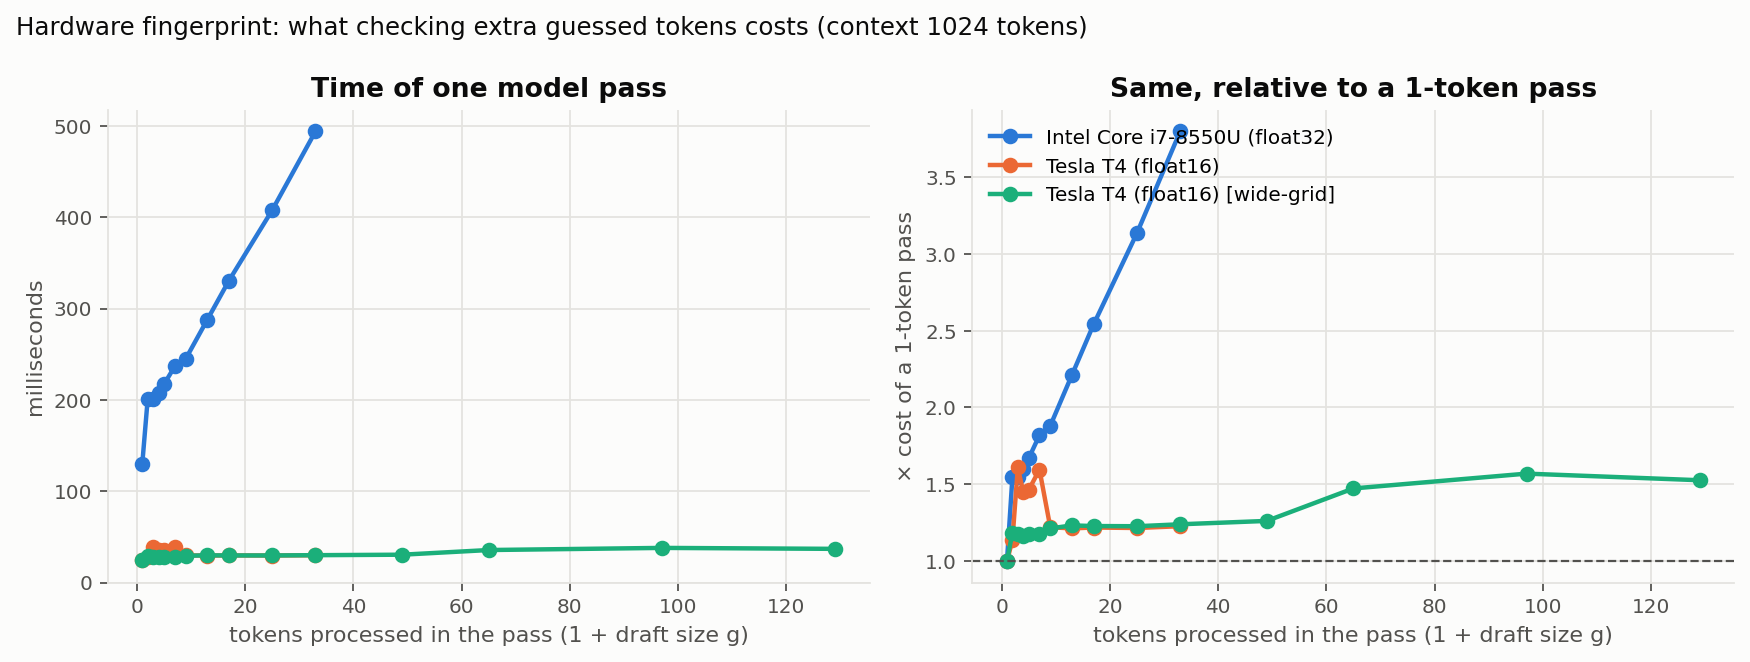
\includegraphics[width=1.00\linewidth]{fig1_hardware_fingerprint.png}
\caption{Hardware fingerprint. Left: time of one forward pass against the number of tokens processed. Right: the same relative to a one-token pass. A flat line means verifying drafted tokens is nearly free.}
\end{figure}
\subsection{Acceptance is device-independent}
\begin{table}[tbp]
\centering
\small
\caption{Tokens gained per pass, $\tau(g)$, on the 12 articles summarised in every run.}
\setlength{\tabcolsep}{4pt}
\begin{tabular}{L{1.13cm}L{4.64cm}L{4.64cm}L{4.64cm}}
\toprule
\textbf{$g$} & \textbf{$\tau$, Intel Core i7-8550U CPU} & \textbf{$\tau$, Tesla T4 GPU} & \textbf{$\tau$, Tesla T4 GPU (extended sweep)} \\
\midrule
1 & 1.48 & 1.48 & 1.48 \\
2 & 1.79 & 1.79 & 1.79 \\
4 & 2.19 & 2.19 & 2.19 \\
8 & 2.60 & 2.60 & 2.60 \\
16 & 3.00 & 3.02 & 3.02 \\
32 & 3.25 & 3.25 & 3.25 \\
\bottomrule
\end{tabular}
\end{table}
On the 12 articles summarised in every run, $\tau$ agrees to within 0.02 at every draft size (Table 3, Figure 2 left), although the devices differ in architecture, precision and speed by more than a factor of four. The remaining differences come from the half-precision near-ties above, which occasionally change the text and with it the acceptance. This confirms the assumption behind both UniSpec's calibration and PPD's split: acceptance can be measured once, and only latency needs to be measured per device.

\subsection{Optimal draft size and the cost of a wrong one}
\begin{table}[tbp]
\centering
\small
\caption{Mean end-to-end speedup over normal decoding by draft size, all articles. Bold: the best draft size of each run.}
\setlength{\tabcolsep}{4pt}
\begin{tabular}{L{2.89cm}L{1.34cm}L{1.34cm}L{1.34cm}L{1.34cm}L{1.34cm}L{1.34cm}L{1.34cm}L{1.34cm}}
\toprule
\textbf{Run} & \textbf{$g$ = 1} & \textbf{$g$ = 2} & \textbf{$g$ = 4} & \textbf{$g$ = 8} & \textbf{$g$ = 16} & \textbf{$g$ = 32} & \textbf{$g$ = 64} & \textbf{$g$ = 128} \\
\midrule
Intel Core i7-8550U CPU & 1.15$\times$ & 1.34$\times$ & 1.51$\times$ & \textbf{1.62$\times$} & 1.61$\times$ & 1.44$\times$ & -- & -- \\
Tesla T4 GPU & 1.33$\times$ & 1.60$\times$ & 1.95$\times$ & 2.31$\times$ & 2.73$\times$ & \textbf{3.17$\times$} & -- & -- \\
Tesla T4 GPU (extended sweep) & 1.34$\times$ & 1.60$\times$ & 1.94$\times$ & 2.42$\times$ & 2.79$\times$ & 3.26$\times$ & 3.56$\times$ & \textbf{4.10$\times$} \\
\bottomrule
\end{tabular}
\end{table}
Because $\tau$ is shared and $s(g)$ is not, the devices want very different draft sizes (Table 4, Figure 2): the Intel Core i7-8550U CPU peaks at $g$ = 8 (1.62$\times$); the Tesla T4 GPU peaks at $g$ = 32 (3.17$\times$), the largest size tried; the Tesla T4 GPU (extended sweep) peaks at $g$ = 128 (4.10$\times$), the largest size tried. On the CPU the speedup falls to 1.44$\times$ at $g$ = 32, and for the 4 articles that copied least from their source $g$ = 32 was slower than normal decoding (0.86$\times$, 0.87$\times$, 0.97$\times$, 0.98$\times$). On the Tesla T4 the curve is still rising at the largest draft size tested: with a 0.5B model the GPU never runs out of spare capacity in this range, so its true optimum may be higher still.

\begin{figure}[tbp]
\centering
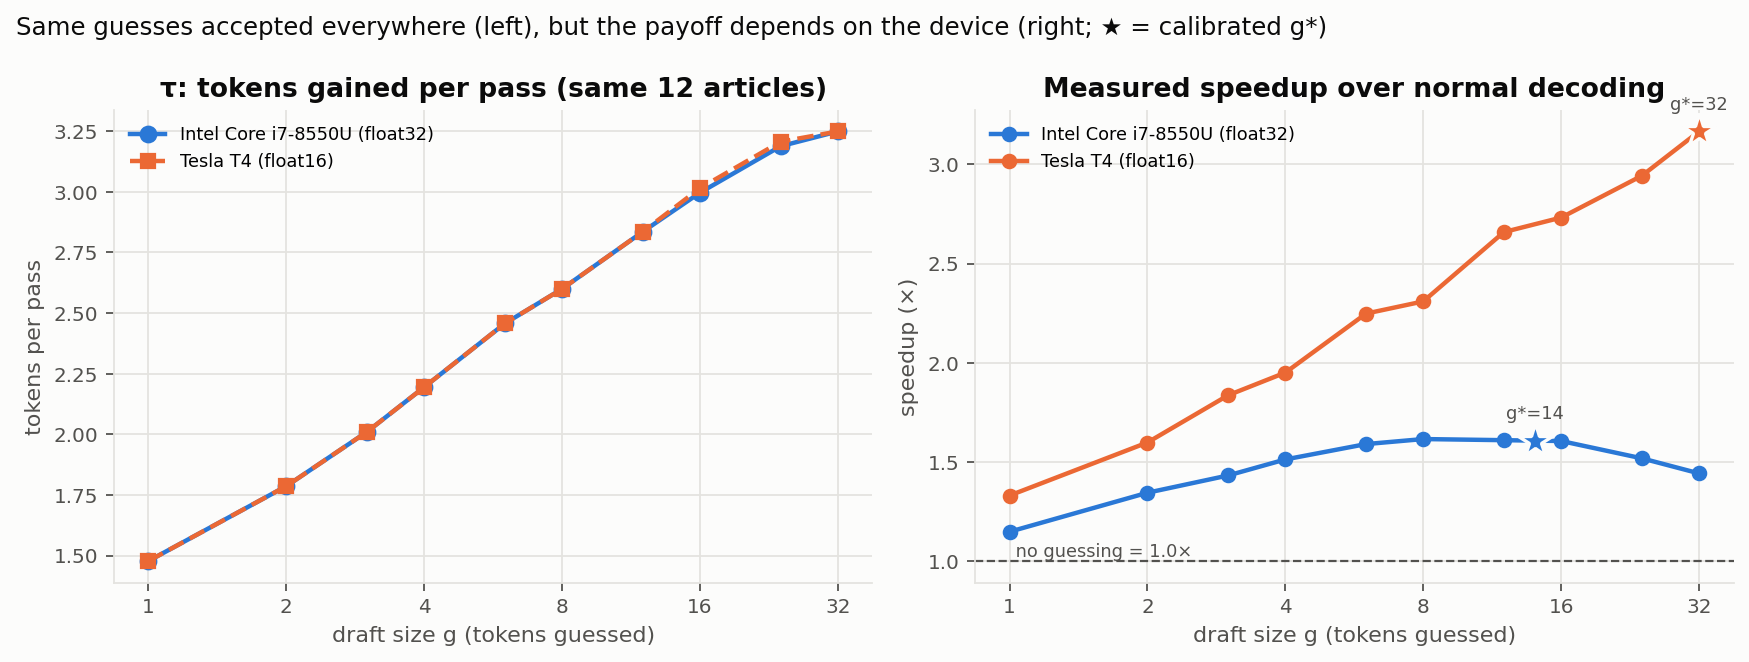
\includegraphics[width=1.00\linewidth]{fig2_draft_size_sweep.png}
\caption{Left: $\tau$ on the articles run on every device; the curves coincide. Right: measured end-to-end speedup by draft size; stars mark each run's calibrated $g^*$. The dashed line is normal decoding.}
\end{figure}
\begin{table}[tbp]
\centering
\small
\caption{Speedup on held-out articles with each run's own calibrated $g^*$ and with a $g^*$ calibrated in another run, read from the run's own sweep (interpolated between tested draft sizes; draft sizes beyond a run's tested range are omitted).}
\setlength{\tabcolsep}{4pt}
\begin{tabular}{L{3.52cm}L{1.47cm}L{1.56cm}L{5.08cm}L{1.56cm}L{1.27cm}}
\toprule
\textbf{Run} & \textbf{Own $g^*$} & \textbf{Speedup} & \textbf{$g^*$ calibrated elsewhere} & \textbf{Speedup} & \textbf{Loss} \\
\midrule
Intel Core i7-8550U CPU & 14 & 1.54$\times$ & 32 (Tesla T4 GPU) & 1.33$\times$ & 13\% \\
Tesla T4 GPU & 32 & 2.36$\times$ & 14 (Intel Core i7-8550U CPU) & 2.22$\times$ & 6\% \\
Tesla T4 GPU (extended sweep) & 128 & 2.45$\times$ & 14 (Intel Core i7-8550U CPU) & 2.12$\times$ & 13\% \\
Tesla T4 GPU (extended sweep) & 128 & 2.45$\times$ & 32 (Tesla T4 GPU) & 2.35$\times$ & 4\% \\
\bottomrule
\end{tabular}
\end{table}
Using a draft size calibrated elsewhere costs speed on every run (Table 5, Figure 3). The CPU loses most, because the GPU's large draft size sits on the steep part of the CPU's cost curve; the GPU loses less because a small draft size only forgoes acceptance it could have had for free. Averaged over articles no run fell below 1.0$\times$ with a foreign draft size, but individual articles did on the CPU, as noted above.

\begin{figure}[tbp]
\centering
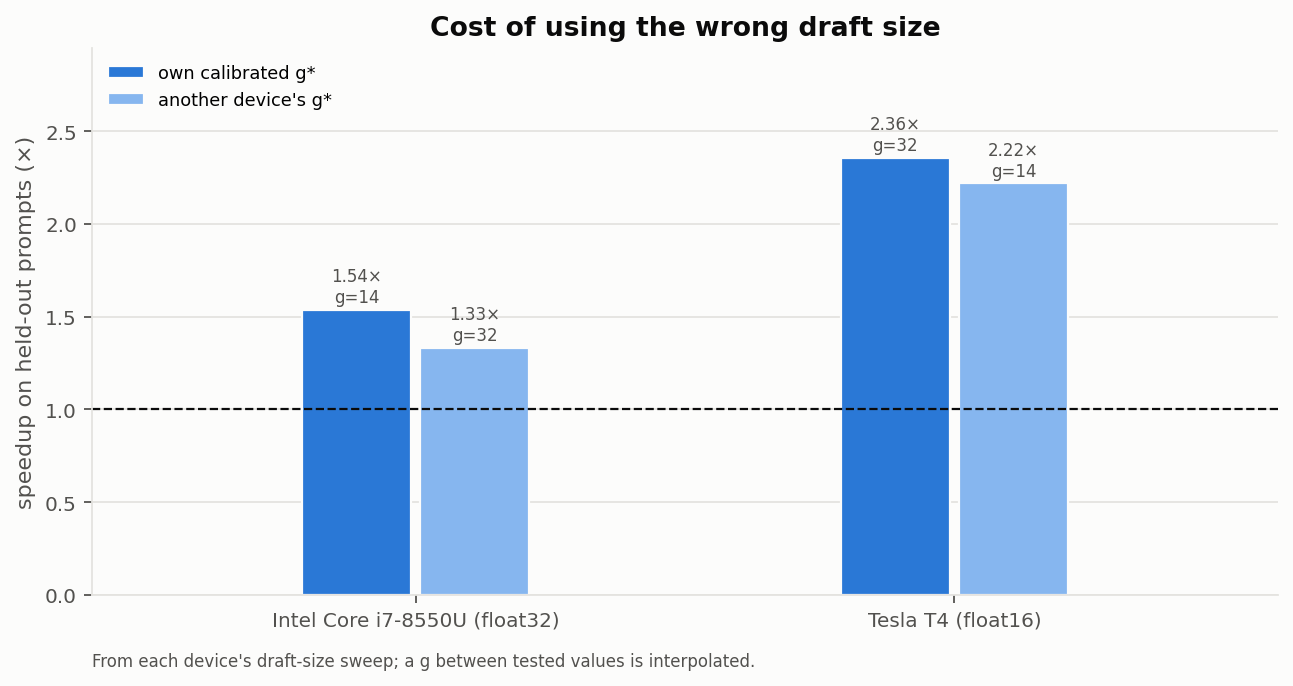
\includegraphics[width=0.90\linewidth]{fig3_wrong_g_cost.png}
\caption{Cost of using the wrong draft size: held-out speedup with each run's own $g^*$ (dark) and with $g^*$ calibrated in another run (light).}
\end{figure}
\subsection{Choosing the draft size automatically}
\begin{table}[tbp]
\centering
\small
\caption{Draft size chosen by each method, the speedup it predicted from the calibration articles, and the speedup measured on held-out articles.}
\setlength{\tabcolsep}{4pt}
\begin{tabular}{L{3.55cm}L{5.41cm}L{1.03cm}L{1.77cm}L{2.99cm}}
\toprule
\textbf{Run} & \textbf{Method} & \textbf{$g^*$} & \textbf{Predicted} & \textbf{Measured (held-out)} \\
\midrule
Intel Core i7-8550U CPU & Grid search & 12 & 1.68$\times$ & 1.47$\times$ \\
Intel Core i7-8550U CPU & UniSpec fit & 14 & 2.23$\times$ & 1.48$\times$ \\
Intel Core i7-8550U CPU & PPD split & 22 & 1.93$\times$ & 1.42$\times$ \\
Intel Core i7-8550U CPU & PPD split, $\tau$ from Tesla T4 GPU & 20 & 2.28$\times$ & 1.38$\times$ \\
Tesla T4 GPU & Grid search & 32 & 3.98$\times$ & 2.36$\times$ \\
Tesla T4 GPU & UniSpec fit & 32 & 4.07$\times$ & 2.36$\times$ \\
Tesla T4 GPU & PPD split & 32 & 3.85$\times$ & 2.36$\times$ \\
Tesla T4 GPU & PPD split, $\tau$ from Intel Core i7-8550U CPU & 32 & 3.06$\times$ & 2.36$\times$ \\
Tesla T4 GPU (extended sweep) & Grid search & 128 & 5.76$\times$ & 2.30$\times$ \\
Tesla T4 GPU (extended sweep) & UniSpec fit & 128 & 6.28$\times$ & 2.30$\times$ \\
Tesla T4 GPU (extended sweep) & PPD split & 128 & 5.86$\times$ & 2.30$\times$ \\
Tesla T4 GPU (extended sweep) & PPD split, $\tau$ from Tesla T4 GPU & 31 & 2.87$\times$ & 2.26$\times$ \\
Tesla T4 GPU (extended sweep) & PPD split, $\tau$ from Intel Core i7-8550U CPU & 7 & 2.39$\times$ & 1.88$\times$ \\
\bottomrule
\end{tabular}
\end{table}
On the Intel Core i7-8550U CPU, measured together in one session on held-out articles, the methods chose $g$ between 12 and 22 and delivered 1.38$\times$--1.48$\times$, within about 10\% of each other, because the CPU's speedup curve is nearly flat around its optimum (Table 6, Figure 4). On the Tesla T4, every method in the first sweep, including the PPD split using $\tau$ measured on the CPU, chose the largest draft size tested, and in the extended sweep UniSpec's fit and grid search again chose the largest size.

Two effects stand out. First, every method over-predicts the speedup, by 14\% for grid search on the CPU and by up to 2.7 times for the UniSpec fit on the extended GPU sweep. Section 5.5 shows why: the speedup depends strongly on how much each article is copied, and the calibration articles happened to copy more than the held-out ones. Second, the PPD split relies on one short synthetic latency profile. On the shared cloud GPU a few profile readings jumped from about 28 to 40 ms; combined with $\tau$ from the CPU, whose sweep stopped at $g$ = 32, the split then chose $g$ = 7 and lost about 18\% against the fit. Methods that time real decoding were not affected.

\begin{figure}[tbp]
\centering
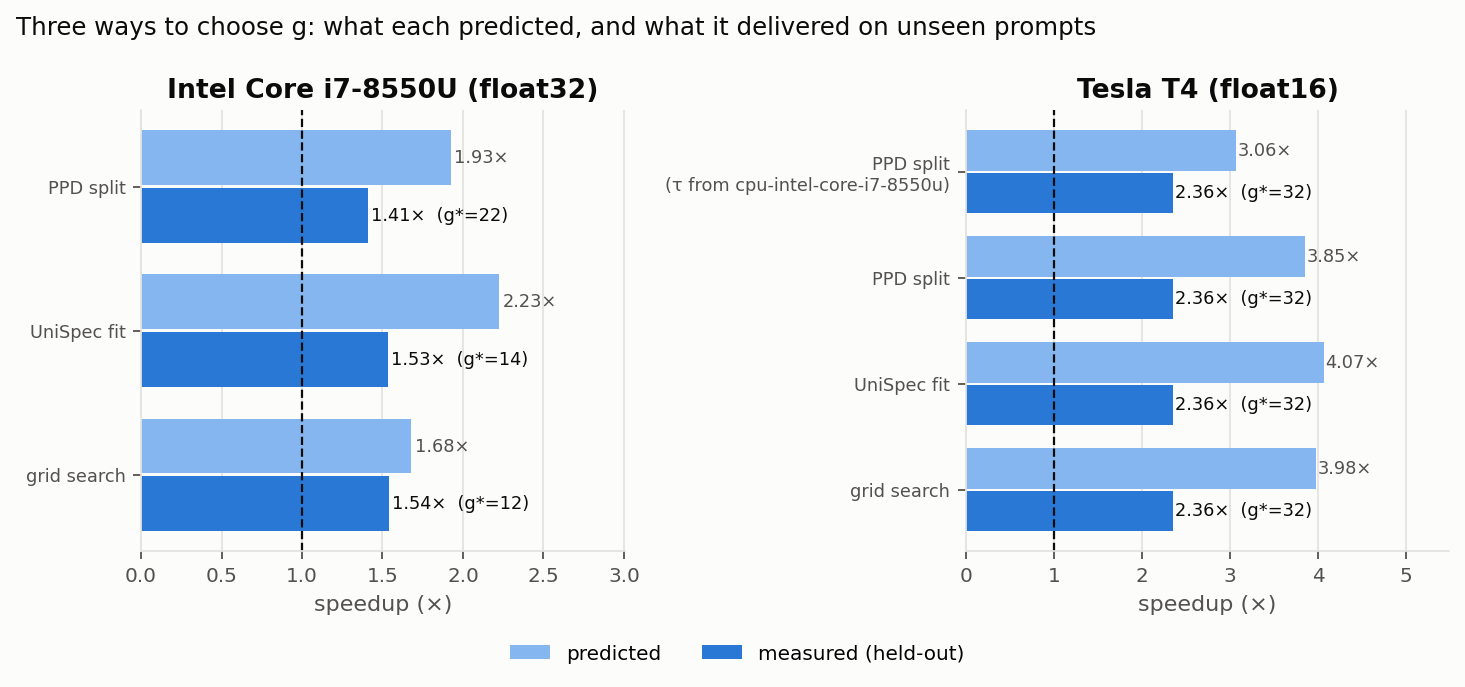
\includegraphics[width=1.00\linewidth]{fig4_calibration_methods.png}
\caption{Calibration methods per run: speedup predicted from the calibration articles (light) and measured on held-out articles (dark), with the chosen $g^*$.}
\end{figure}
\subsection{Copying drives the speedup}
Across articles the speedup varies widely, and the share of the summary copied from the article explains most of that variation (Figure 5). At $g$ = 8 the Pearson correlation between copy share and generation-only speedup is $r$ = 0.85 over 32 articles on the Intel Core i7-8550U CPU; $r$ = 0.85 over 115 articles on the Tesla T4 GPU; $r$ = 0.87 over 30 articles on the Tesla T4 GPU (extended sweep). On the CPU, English summaries that copy about 20\% of their 4-token sequences run about 1.1$\times$ faster, while those that copy 90\% run about 3.4$\times$ faster. The calibration articles copied 54\% on average and the held-out articles 50\%, consistent with the over-prediction in Section 5.4. For a retrieval drafter, the task decides how much can be gained and the hardware decides how large $g$ can usefully be.

\begin{figure}[tbp]
\centering
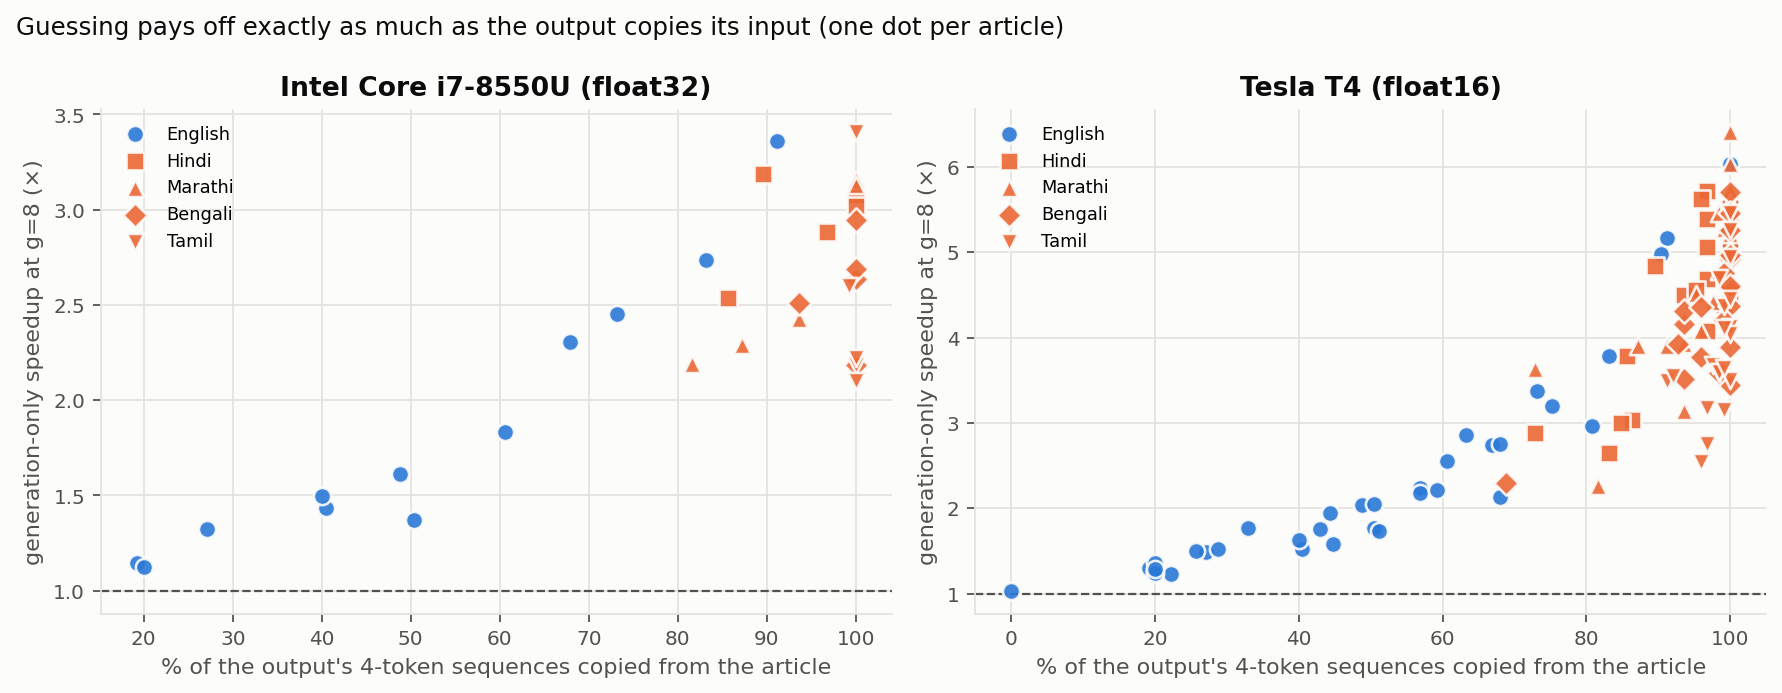
\includegraphics[width=1.00\linewidth]{fig7_copying_vs_speedup.png}
\caption{Generation-only speedup at $g$ = 8 against the share of the summary's 4-token sequences that also occur in the article; one point per article, marker shape by language.}
\end{figure}
\subsection{Indian languages}
\begin{table}[tbp]
\centering
\small
\caption{Tokenizer granularity on the 250-word article excerpts, and the resulting mean prompt length for Qwen2.5 (including instructions).}
\setlength{\tabcolsep}{4pt}
\begin{tabular}{L{2.60cm}L{4.20cm}L{4.20cm}L{3.40cm}}
\toprule
\textbf{Language} & \textbf{Tokens per word, Qwen2.5-0.5B-Instruct} & \textbf{Tokens per word, sarvam-1} & \textbf{Prompt length (tokens)} \\
\midrule
English & 1.27 & 1.47 & 366 \\
Hindi & 4.70 & 1.40 & 1,220 \\
Marathi & 6.64 & 1.88 & 1,643 \\
Bengali & 7.02 & 1.85 & 1,818 \\
Tamil & 10.09 & 2.26 & 2,571 \\
\bottomrule
\end{tabular}
\end{table}
Qwen2.5's tokenizer splits the Indian languages into 4.7--10.1 tokens per word against 1.27 for English (Table 7). The tokenizer of Sarvam-1, a model built for Indian languages, needs only 1.4--2.3 tokens per word for the same text, so the difference lies in the tokenizer rather than in the languages. As a result a 250-word Tamil excerpt becomes a prompt about seven times longer than its English counterpart.

\begin{table}[tbp]
\centering
\small
\caption{Language study on held-out articles at each device's calibrated draft size. Copied and repeated: share of the summary's 4-token sequences found in the article and earlier in the summary. Prefill is the time normal decoding spends reading the prompt.}
\setlength{\tabcolsep}{4pt}
\begin{tabular}{L{2.76cm}L{1.65cm}L{1.38cm}L{1.65cm}L{1.01cm}L{2.11cm}L{1.75cm}L{1.56cm}}
\toprule
\textbf{Run} & \textbf{Language} & \textbf{Copied} & \textbf{Repeated} & \textbf{$\tau$} & \textbf{Generation only} & \textbf{End to end} & \textbf{Prefill (s)} \\
\midrule
Intel Core i7-8550U, $g$ = 14 & English & 56\% & 0\% & 2.85 & 1.90$\times$ & 1.64$\times$ & 2.78 \\
Intel Core i7-8550U, $g$ = 14 & Hindi & 94\% & 5\% & 8.37 & 3.92$\times$ & 1.90$\times$ & 8.50 \\
Intel Core i7-8550U, $g$ = 14 & Marathi & 92\% & 12\% & 6.73 & 2.99$\times$ & 1.64$\times$ & 11.28 \\
Intel Core i7-8550U, $g$ = 14 & Bengali & 99\% & 9\% & 8.45 & 3.57$\times$ & 1.68$\times$ & 12.66 \\
Intel Core i7-8550U, $g$ = 14 & Tamil & 100\% & 6\% & 6.92 & 2.73$\times$ & 1.42$\times$ & 20.14 \\
Tesla T4, $g$ = 32 & English & 42\% & 3\% & 2.46 & 2.27$\times$ & 2.23$\times$ & 0.03 \\
Tesla T4, $g$ = 32 & Hindi & 94\% & 4\% & 12.10 & 10.16$\times$ & 8.55$\times$ & 0.06 \\
Tesla T4, $g$ = 32 & Marathi & 95\% & 7\% & 11.85 & 9.58$\times$ & 7.44$\times$ & 0.09 \\
Tesla T4, $g$ = 32 & Bengali & 97\% & 7\% & 12.61 & 10.10$\times$ & 7.70$\times$ & 0.10 \\
Tesla T4, $g$ = 32 & Tamil & 98\% & 12\% & 9.76 & 7.47$\times$ & 5.63$\times$ & 0.15 \\
\bottomrule
\end{tabular}
\end{table}
Our proposal predicted that more pieces per word would make tokens harder to guess and lower acceptance. The opposite happened (Table 8, Figure 6). Two effects combine. The 0.5B model largely copies the article when summarising in these languages: 92\%--100\% of its 4-token sequences come from the article, against about half in English, while self-repetition stays low. And each copied word is many tokens long, so a single correct guess of a word yields many tokens at once.

How much of that gain survives end to end depends on how fast the device reads the prompt. On the Tesla T4, generation alone became 7.47$\times$--10.16$\times$ faster for the Indian languages and whole requests 5.63$\times$--8.55$\times$ faster. On the Intel Core i7-8550U, generation alone was 2.73$\times$--3.92$\times$ faster, but whole requests only 1.42$\times$--1.90$\times$. Reading a Tamil prompt takes 20.1 s of a 39.6 s request on the CPU but 0.15 s on the GPU. Fine-grained tokenization thus helps acceptance and hurts prefill, and the hardware decides which effect dominates.

The model's summaries in these languages are of low quality and heavily extractive. Decoding is lossless, so this does not affect the speed comparison, but a larger model that paraphrases more would likely accept fewer drafted tokens.

\begin{figure}[tbp]
\centering
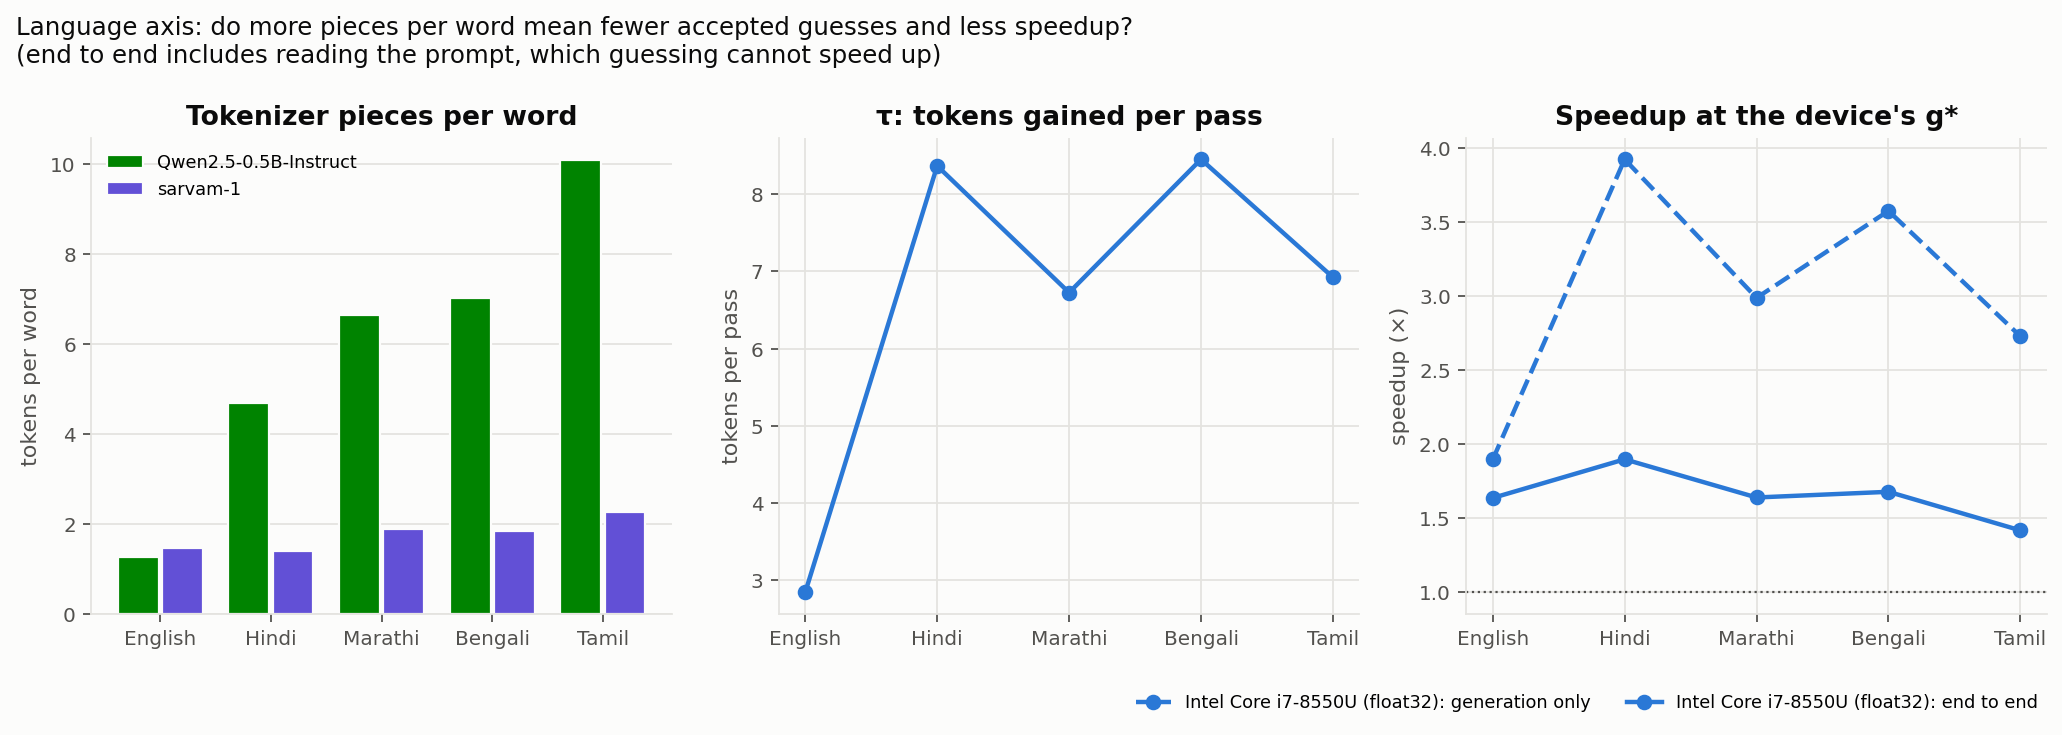
\includegraphics[width=1.00\linewidth]{fig5_language.png}
\caption{Languages. Left: tokens per word for two tokenizers. Middle: $\tau$ at each device's calibrated draft size. Right: speedup at that draft size, end to end (solid) and generation only (dashed).}
\end{figure}
\subsection{Sustained load}
\begin{table}[tbp]
\centering
\small
\caption{Sustained load on the Intel Core i7-8550U CPU: each cycle covers every held-out article once, so article content averages out.}
\setlength{\tabcolsep}{4pt}
\begin{tabular}{L{1.25cm}L{1.93cm}L{2.51cm}L{2.60cm}L{3.28cm}L{2.89cm}}
\toprule
\textbf{Cycle} & \textbf{Minutes} & \textbf{1-token pass (ms)} & \textbf{15-token pass (ms)} & \textbf{Normal decoding (tokens/s)} & \textbf{Speedup at $g$ = 14} \\
\midrule
1 & 0.8--4.2 & 155 & 355 & 5.8 & 1.45$\times$ \\
2 & 5.0--8.3 & 157 & 348 & 5.9 & 1.49$\times$ \\
3 & 9.1--12.2 & 144 & 329 & 6.2 & 1.47$\times$ \\
4 & 13.0--16.2 & 151 & 326 & 6.0 & 1.51$\times$ \\
5 & 17.0--20.3 & 157 & 351 & 5.9 & 1.49$\times$ \\
\bottomrule
\end{tabular}
\end{table}
Over 20 minutes of continuous work on the plugged-in Intel Core i7-8550U CPU, pass times and the speedup at the calibrated $g$ = 14 showed no downward trend: the per-cycle speedup stayed between 1.45$\times$ and 1.51$\times$ (Table 9, Figure 7). The raw per-round speedup varies between about 1.0$\times$ and 2.1$\times$, but that is the articles taking turns, which is why the table averages over full cycles.

Power state mattered more than heat. In a separate short run on battery power the same laptop needed about 197 ms per normal pass instead of 124 ms. A draft size calibrated on mains power is then applied to a different cost curve, which is the kind of instability UniSpec's limitations anticipate. Our software therefore detects battery operation and stores such runs separately.

\begin{figure}[tbp]
\centering
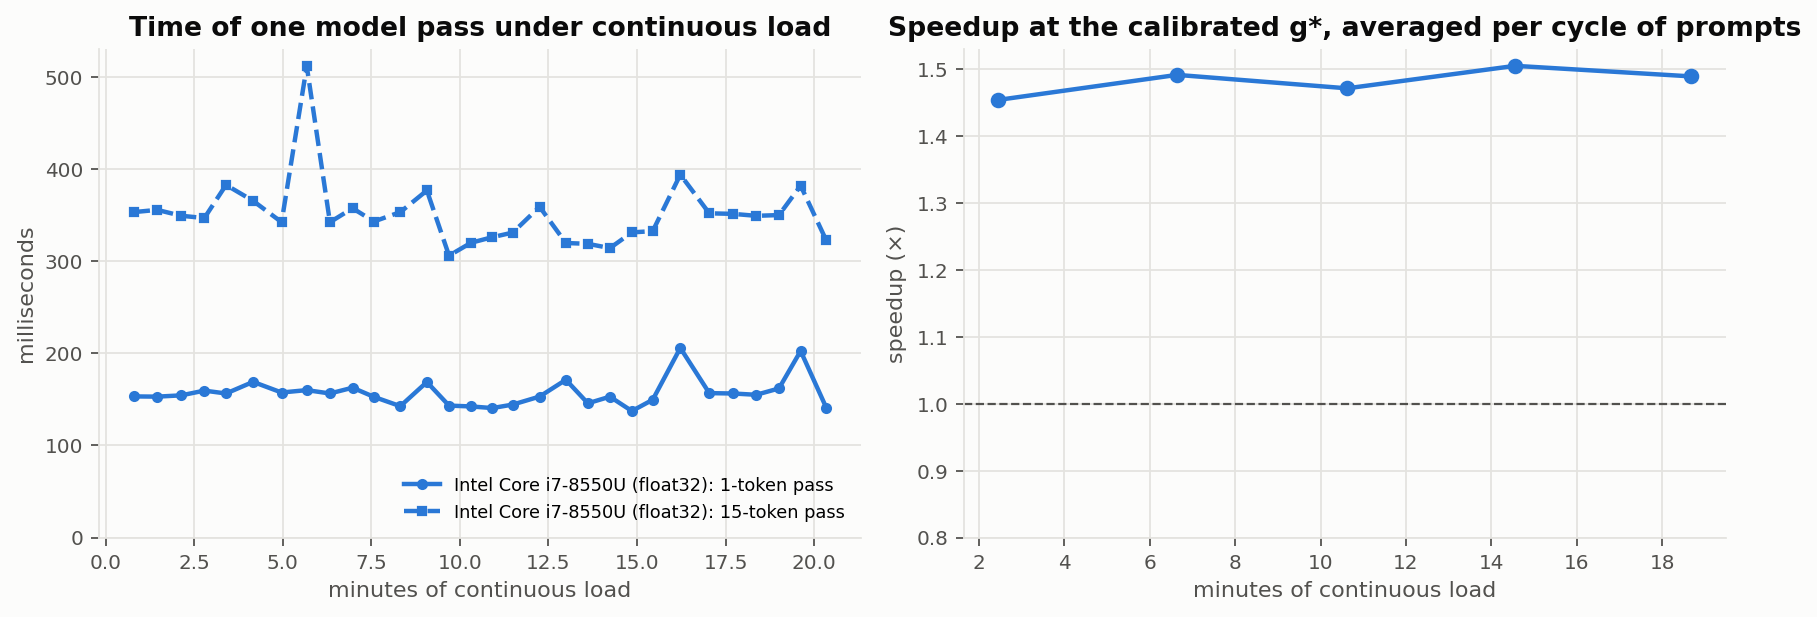
\includegraphics[width=1.00\linewidth]{fig6_thermal.png}
\caption{Sustained load. Left: one-token and $(1+g^*)$-token pass times over 20 minutes. Right: speedup at the calibrated $g^*$, averaged per cycle of held-out articles.}
\end{figure}
\section{Discussion}
\textbf{The shared rule holds and its split is practical.} Acceptance matched across a 32-bit CPU and a 16-bit GPU, so $\tau$ can be measured once on any machine and only the latency curve, a two-minute measurement, has to be repeated per device. This is the practical value of PPD's decomposition for anyone without long access to the target hardware.

\textbf{Everyday hardware sits at the far end of the cost curve.} UniSpec observes smaller optimal draft sizes on consumer GPUs than on data-centre GPUs. The laptop CPU extends that trend: beyond the first extra token, verification cost grows almost linearly with the draft size, the optimum falls to around 8--16, and a draft size suited to a GPU loses 14\% and can make individual requests slower than no speculation at all. The free T4, in contrast, still had idle capacity at $g$ = 128, because a 0.5B model leaves it memory-bound; with UniSpec's 8B--14B models its optimum would be lower.

\textbf{Calibration selects well but predicts poorly.} Because the speedup curves are flat near their optimum, every reasonable method chose a draft size close to the best. The predicted speedups, however, ranged from 14\% too high to 2.7 times the measured value, because acceptance depends on how much each input is copied and a handful of calibration articles does not represent that well. A deployment should calibrate on inputs typical of its own workload and treat the predicted speedup as an upper estimate.

\textbf{Profile-only calibration needs repeated measurements on shared hardware.} The PPD split rests on a single synthetic latency profile. On a shared cloud GPU, transient slowdowns in a few readings moved its choice from the largest draft size to $g$ = 7. Repeating the profile and taking the median per size, or timing real decoding as UniSpec does, avoids this.

\textbf{Tokenization decides the language result.} Fine-grained tokenization of Indian scripts is not a barrier to n-gram speculation: copied words become long, easily guessed runs of tokens. It is a barrier to latency on devices with slow prefill, because the same text costs several times more tokens to read. A tokenizer built for these languages, such as Sarvam-1's, would shorten prompts by a similar factor and remove most of that cost.

\section{Limitations}
\begin{itemize}
  \item \textbf{Simplified UniSpec.} A single chain of drafted tokens replaces confidence-scored draft trees; we evaluate UniSpec's calibration, not its full drafter, so absolute speedups are not comparable with the paper.
  \item \textbf{No PPD drafter.} Its prompt-token embeddings require GPU training beyond our budget.
  \item \textbf{One small model.} Qwen2.5-0.5B is far smaller than the papers' 7B--14B models. Larger models load the GPU more and would lower its optimal draft size; on a CPU they would make every pass slower.
  \item \textbf{Few devices.} 2 devices so far. The benchmark runs unchanged on further CPUs and GPUs, and their results join every table and figure of this report on rebuilding.
  \item \textbf{Timing noise.} Laptop and shared-GPU timings are noisier than dedicated servers. Paired back-to-back runs, held-out articles and single-session comparisons reduce this, but differences below about 5\% should not be over-interpreted.
  \item \textbf{Indian-language quality.} The small model copies heavily in these languages; acceptance is likely lower with stronger models.
\end{itemize}
\section{Conclusion}
The hardware-aware rule shared by UniSpec and PPD transfers to everyday hardware: acceptance is device-independent, latency is not, and measuring latency per device selects a good draft size. The optimal draft size differs by an order of magnitude between a laptop CPU (8) and a free cloud GPU (128 or more), and using the wrong one costs 6--14\% on average and can make individual requests slower than normal decoding. Calibration chooses well but over-promises, because the gain depends as much on how much the output copies its input as on the hardware. In Indian languages, fine-grained tokenization raises acceptance, up to 8.55$\times$ end to end on the GPU, but lengthens prompts so much that on a CPU reading them limits the gain to 1.42$\times$--1.90$\times$.

\begin{thebibliography}{99}
\addcontentsline{toc}{section}{References}
\small
\bibitem{unispec} D.-T. Do, N.-K. Le, and N. L. Minh. UniSpec: Training-free speculative decoding for robust LLM acceleration across languages and hardware. In \emph{Proceedings of the 64th Annual Meeting of the Association for Computational Linguistics (ACL)}, pages 6288--6310, 2026. \url{https://aclanthology.org/2026.acl-long.285/}
\bibitem{ppd} H. Chen, W. Luk, K. F. C. Yiu, R. Li, K. Mishchenko, S. I. Venieris, and H. Fan. Hardware-aware parallel prompt decoding for memory-efficient acceleration of LLM inference. In \emph{Findings of the Association for Computational Linguistics: EMNLP 2025}, pages 2221--2238, 2025. \url{https://aclanthology.org/2025.findings-emnlp.120/}
\bibitem{leviathan} Y. Leviathan, M. Kalman, and Y. Matias. Fast inference from transformers via speculative decoding. In \emph{Proceedings of the 40th International Conference on Machine Learning (ICML)}, 2023.
\bibitem{chen} C. Chen, S. Borgeaud, G. Irving, J.-B. Lespiau, L. Sifre, and J. Jumper. Accelerating large language model decoding with speculative sampling. arXiv:2302.01318, 2023.
\bibitem{medusa} T. Cai, Y. Li, Z. Geng, H. Peng, J. D. Lee, D. Chen, and T. Dao. Medusa: Simple LLM inference acceleration framework with multiple decoding heads. In \emph{Proceedings of the 41st International Conference on Machine Learning (ICML)}, 2024.
\bibitem{eagle} Y. Li, F. Wei, C. Zhang, and H. Zhang. EAGLE: Speculative sampling requires rethinking feature uncertainty. In \emph{Proceedings of the 41st International Conference on Machine Learning (ICML)}, 2024.
\bibitem{lookahead} Y. Fu, P. Bailis, I. Stoica, and H. Zhang. Break the sequential dependency of LLM inference using lookahead decoding. In \emph{Proceedings of the 41st International Conference on Machine Learning (ICML)}, 2024.
\bibitem{pld} A. Saxena. Prompt lookup decoding. Software, \url{https://github.com/apoorvumang/prompt-lookup-decoding}, 2023.
\bibitem{rest} Z. He, Z. Zhong, T. Cai, J. D. Lee, and D. He. REST: Retrieval-based speculative decoding. In \emph{Proceedings of NAACL-HLT}, 2024.
\bibitem{specinfer} X. Miao et al. SpecInfer: Accelerating large language model serving with tree-based speculative inference and verification. In \emph{Proceedings of ASPLOS}, 2024.
\bibitem{sequoia} Z. Chen, A. May, R. Svirschevski, Y. Huang, M. Ryabinin, Z. Jia, and B. Chen. Sequoia: Scalable, robust, and hardware-aware speculative decoding. arXiv:2402.12374, 2024.
\bibitem{specbench} H. Xia, Z. Yang, Q. Dong, P. Wang, Y. Li, T. Ge, T. Liu, W. Li, and Z. Sui. Unlocking efficiency in large language model inference: A comprehensive survey of speculative decoding. In \emph{Findings of the Association for Computational Linguistics: ACL 2024}, 2024.
\bibitem{roofline} S. Williams, A. Waterman, and D. Patterson. Roofline: An insightful visual performance model for multicore architectures. \emph{Communications of the ACM}, 52(4):65--76, 2009.
\bibitem{vllm} W. Kwon, Z. Li, S. Zhuang, Y. Sheng, L. Zheng, C. H. Yu, J. E. Gonzalez, H. Zhang, and I. Stoica. Efficient memory management for large language model serving with PagedAttention. In \emph{Proceedings of the 29th Symposium on Operating Systems Principles (SOSP)}, 2023.
\bibitem{xlsum} T. Hasan, A. Bhattacharjee, M. S. Islam, K. Mubasshir, Y.-F. Li, Y.-B. Kang, M. S. Rahman, and R. Shahriyar. XL-Sum: Large-scale multilingual abstractive summarization for 44 languages. In \emph{Findings of the Association for Computational Linguistics: ACL-IJCNLP 2021}, 2021.
\bibitem{qwen} Qwen Team. Qwen2.5 technical report. arXiv:2412.15115, 2024.
\bibitem{de} R. Storn and K. Price. Differential evolution: A simple and efficient heuristic for global optimization over continuous spaces. \emph{Journal of Global Optimization}, 11(4):341--359, 1997.
\bibitem{transformers} T. Wolf et al. Transformers: State-of-the-art natural language processing. In \emph{Proceedings of EMNLP: System Demonstrations}, 2020.
\bibitem{pytorch} A. Paszke et al. PyTorch: An imperative style, high-performance deep learning library. In \emph{Advances in Neural Information Processing Systems (NeurIPS)}, 2019.
\end{thebibliography}
\clearpage
\appendix
\section{Draft-size sweeps in full}
\begin{table}[H]
\centering
\small
\caption{Draft-size sweep on the Intel Core i7-8550U CPU, all articles ($g$ = 0 is normal decoding).}
\setlength{\tabcolsep}{4pt}
\begin{tabular}{L{0.99cm}L{1.25cm}L{1.61cm}L{2.06cm}L{2.06cm}L{1.70cm}L{2.33cm}L{1.88cm}}
\toprule
\textbf{$g$} & \textbf{$\tau$} & \textbf{Accepted} & \textbf{Tokens per pass} & \textbf{Pass time (ms)} & \textbf{Speedup} & \textbf{Generation-only} & \textbf{Exact match} \\
\midrule
0 & 1.00 & 0\% & 1.0 & 124.3 & 1.00$\times$ & 1.00$\times$ & 100\% \\
1 & 1.48 & 75\% & 1.6 & 156.3 & 1.15$\times$ & 1.17$\times$ & 100\% \\
2 & 1.79 & 67\% & 2.1 & 154.5 & 1.34$\times$ & 1.43$\times$ & 100\% \\
3 & 2.01 & 60\% & 2.5 & 157.8 & 1.43$\times$ & 1.57$\times$ & 100\% \\
4 & 2.19 & 56\% & 2.9 & 158.7 & 1.51$\times$ & 1.70$\times$ & 100\% \\
6 & 2.46 & 47\% & 3.7 & 162.8 & 1.59$\times$ & 1.84$\times$ & 100\% \\
8 & 2.60 & 41\% & 4.4 & 168.5 & 1.62$\times$ & 1.85$\times$ & 100\% \\
12 & 2.84 & 34\% & 5.7 & 181.4 & 1.61$\times$ & 1.88$\times$ & 100\% \\
16 & 3.00 & 28\% & 7.1 & 187.2 & 1.61$\times$ & 1.91$\times$ & 100\% \\
24 & 3.19 & 22\% & 9.4 & 212.8 & 1.52$\times$ & 1.78$\times$ & 100\% \\
32 & 3.25 & 18\% & 11.8 & 231.1 & 1.44$\times$ & 1.66$\times$ & 100\% \\
\bottomrule
\end{tabular}
\end{table}
\begin{table}[H]
\centering
\small
\caption{Draft-size sweep on the Tesla T4 GPU, all articles ($g$ = 0 is normal decoding).}
\setlength{\tabcolsep}{4pt}
\begin{tabular}{L{0.99cm}L{1.25cm}L{1.61cm}L{2.06cm}L{2.06cm}L{1.70cm}L{2.33cm}L{1.88cm}}
\toprule
\textbf{$g$} & \textbf{$\tau$} & \textbf{Accepted} & \textbf{Tokens per pass} & \textbf{Pass time (ms)} & \textbf{Speedup} & \textbf{Generation-only} & \textbf{Exact match} \\
\midrule
0 & 1.00 & 0\% & 1.0 & 26.2 & 1.00$\times$ & 1.00$\times$ & 100\% \\
1 & 1.47 & 75\% & 1.6 & 28.8 & 1.33$\times$ & 1.33$\times$ & 93\% \\
2 & 1.77 & 65\% & 2.1 & 28.7 & 1.60$\times$ & 1.61$\times$ & 90\% \\
3 & 2.00 & 59\% & 2.5 & 28.0 & 1.84$\times$ & 1.85$\times$ & 90\% \\
4 & 2.18 & 54\% & 2.9 & 28.6 & 1.95$\times$ & 1.97$\times$ & 90\% \\
6 & 2.46 & 46\% & 3.7 & 27.8 & 2.25$\times$ & 2.28$\times$ & 90\% \\
8 & 2.65 & 40\% & 4.4 & 28.9 & 2.31$\times$ & 2.35$\times$ & 90\% \\
12 & 2.94 & 33\% & 5.8 & 27.8 & 2.66$\times$ & 2.72$\times$ & 90\% \\
16 & 3.16 & 28\% & 7.2 & 29.1 & 2.73$\times$ & 2.81$\times$ & 93\% \\
24 & 3.45 & 23\% & 9.7 & 28.9 & 2.94$\times$ & 3.06$\times$ & 93\% \\
32 & 3.74 & 19\% & 12.1 & 29.0 & 3.17$\times$ & 3.34$\times$ & 97\% \\
\bottomrule
\end{tabular}
\end{table}
\begin{table}[H]
\centering
\small
\caption{Draft-size sweep on the Tesla T4 GPU (extended sweep), all articles ($g$ = 0 is normal decoding).}
\setlength{\tabcolsep}{4pt}
\begin{tabular}{L{0.99cm}L{1.25cm}L{1.61cm}L{2.06cm}L{2.06cm}L{1.70cm}L{2.33cm}L{1.88cm}}
\toprule
\textbf{$g$} & \textbf{$\tau$} & \textbf{Accepted} & \textbf{Tokens per pass} & \textbf{Pass time (ms)} & \textbf{Speedup} & \textbf{Generation-only} & \textbf{Exact match} \\
\midrule
0 & 1.00 & 0\% & 1.0 & 26.3 & 1.00$\times$ & 1.00$\times$ & 100\% \\
1 & 1.47 & 75\% & 1.6 & 28.5 & 1.34$\times$ & 1.35$\times$ & 93\% \\
2 & 1.77 & 65\% & 2.1 & 28.8 & 1.60$\times$ & 1.61$\times$ & 90\% \\
4 & 2.18 & 54\% & 2.9 & 29.0 & 1.94$\times$ & 1.96$\times$ & 90\% \\
8 & 2.65 & 40\% & 4.4 & 27.8 & 2.42$\times$ & 2.47$\times$ & 90\% \\
16 & 3.16 & 28\% & 7.2 & 28.4 & 2.79$\times$ & 2.87$\times$ & 93\% \\
32 & 3.74 & 19\% & 12.1 & 28.1 & 3.26$\times$ & 3.43$\times$ & 97\% \\
48 & 4.03 & 15\% & 16.1 & 28.6 & 3.38$\times$ & 3.63$\times$ & 93\% \\
64 & 4.42 & 13\% & 19.7 & 28.7 & 3.56$\times$ & 3.92$\times$ & 90\% \\
96 & 4.48 & 11\% & 24.6 & 28.1 & 3.72$\times$ & 4.11$\times$ & 90\% \\
128 & 5.22 & 10\% & 27.3 & 28.3 & 4.10$\times$ & 4.88$\times$ & 93\% \\
\bottomrule
\end{tabular}
\end{table}
\section{Fitted calibration models}
\begin{table}[H]
\centering
\small
\caption{Parameters of the UniSpec-style fits of Equation 2 on the calibration articles. The continuous optimum is found by Differential Evolution and rounded to the better neighbouring integer.}
\setlength{\tabcolsep}{4pt}
\begin{tabular}{L{3.29cm}L{1.10cm}L{1.10cm}L{1.46cm}L{1.46cm}L{1.73cm}L{2.01cm}L{1.73cm}}
\toprule
\textbf{Run} & \textbf{$a$} & \textbf{$b$} & \textbf{$c_0$ (ms)} & \textbf{$c_1$ (ms)} & \textbf{$c_2$ (ms)} & \textbf{Continuous $g^*$} & \textbf{Integer $g^*$} \\
\midrule
Intel Core i7-8550U CPU & 2.71 & 6.46 & 152.53 & 2.922 & -0.00553 & 13.9 & 14 \\
Tesla T4 GPU & 3.76 & 9.29 & 28.22 & 0.082 & -0.00154 & 32.0 & 32 \\
Tesla T4 GPU (extended sweep) & 5.81 & 25.13 & 28.73 & -0.009 & 0.00002 & 128.0 & 128 \\
\bottomrule
\end{tabular}
\end{table}
\section{Reproducing and extending the results}
Code, the fixed article subset, raw results, figures and this report's generator are in the project repository: \url{https://github.com/AdityaRaj272/unispec-everyday-hardware-indic}. On any machine with Python 3.9 or newer:

\begin{lstlisting}
pip install -r requirements.txt
python tests/test_engine.py            # engine correctness with a mock model
python run.py all                      # every benchmark on this machine
python run.py thermal --minutes 20     # sustained load (laptops)
python run.py plots                    # figures and results/SUMMARY.md
python report/build_report.py          # this report, rebuilt from results/
\end{lstlisting}
The device, number precision and workload are detected automatically, and a laptop on battery is recorded as a separate run. To add a device, run the benchmark on it, copy its results folder into results/, and rebuild the figures and this report: every table and figure includes the new run. GPU results here were produced with notebooks/colab\_t4.ipynb on Google Colab's free T4.

\end{document}
